\chapter{Introducción}

 
La ciencia de ondas gravitacionales es un área que ha experimentado un rápido crecimiento en las últimas décadas. Este crecimiento llevó, en septiembre de 2015, a la primera detección obtenida de ondas gravitacionales producto de una colisión binaria de agujeros negros \cite{https://doi.org/10.48550/arxiv.1607.05251, LIGOScientific:2016aoc}. Al momento de escribir esta tesis (últimos meses de 2022), los interferómetros LIGO, VIRGO y KAGRA van detectando cerca de 50 eventos, y planean empezar la cuarta serie de observaciones O4 a mediados de mayo de 2023 \footnote{\url{https://observing.docs.ligo.org/plan/}}.


Cada observación no solo confirma una de las predicciones más relevantes de las ecuaciones de Einstein, sino que también aporta una gran cantidad de información sobre los fenómenos que las producen. De una onda producida por la colisión de dos agujeros negros se pueden inferir un total de 15 parámetros, de los cuales algunos son \textit{intrínsecos} (como la relación entre las masas o los espines) y otros \textit{extrínsecos} (la distancia del evento, la posición en el cielo, etc.) \cite{Veitch_2015}.


La estimación de parámetros se realiza utilizando inferencia Bayesiana \cite{Thrane_2019}, un método que requiere generar funciones de onda para diversos parámetros en tiempo real. Esto es un problema debido a la dificultad que representa resolver las ecuaciones de Einstein; ya que utilizando relatividad numérica se necesitan meses de cómputo para obtener la función de onda producto de una colisión binaria. Debido a que se necesitan varias configuraciones al momento de realizar la inferencia de parámetros, la relatividad numérica no es una opción a la hora de generar las funciones de onda. 

En esta tesis se trabajó dentro del marco de los modelos sustitutos de orden reducido \cite{Field_2014, Tiglio:2021ysj}, una alternativa que logra generar soluciones de alta precisión, comparables a los métodos de relatividad numérica, pero en tiempo real y en una simple computadora portátil. Dentro de este marco se utilizó el enfoque de las bases reducidas \cite{rb0book, doi:10.1137/09075250X, PhysRevLett.106.221102, 10.1115/1.1448332, rb1book}, un método espectral que permite representar un espacio de soluciones a partir de sus $n$ elementos más representativos, de forma que se elimina la información redundante a la hora de representar dicho espacio.


\subsection*{Objetivo}

En este trabajo se expande el método de bases reducidas con el refinamiento \textit{hp-greedy} \cite{Cerino:2022dhr}, el cual divide iterativamente el espacio de parámetros en distintos subdominios, construyendo bases reducidas locales en lugar de una global, y dando como resultado una estructura de árbol binario.

La ventaja de este refinamiento está en que las bases locales tienen menor dimensión que la base global, sin que esto implique una pérdida de precisión. Esto se traduce en un modelo más rápido y eficiente de evaluar, pues en lugar de representar una solución proyectándola a la base global, se la proyectará a una de las bases locales (la que corresponda según los parámetros de la solución). 
Pero junto a esta ventaja se agrega la complejidad de los hiperparámetros que gobiernan la construcción de esta base (por ejemplo, la profundidad máxima del árbol).


El objetivo de esta tesis es encontrar la configuración de hiperparámetros que de lugar a una base óptima. Partiendo de un espacio de hiperparámetros, una base reducida \textit{hp-greedy} óptima será aquella con la configuración de hiperparámetros que de lugar al menor error de representación a la hora de proyectar un dado espacio. 

%Por lo que el problema de obtener una base óptima implica obtener una configuración óptima de hiperparámetros, la cual es una tarea complicada y que no se puede resolver por fuerza bruta debido al alto número de configuraciones existentes. Es por esta razón que surge la necesidad de utilizar métodos de optimización.

\subsection*{Metodología: Optimización Bayesiana}

Una base reducida \textit{hp-greedy} constituye un sistema de aprendizaje supervisado con numerosas configuraciones de hiperparámetros, cuyo ajuste afecta significativamente el rendimiento del sistema. Por lo tanto, resulta fundamental optimizar la construcción de este sistema.

La optimización bayesiana \cite{7352306, https://doi.org/10.48550/arxiv.1012.2599} se ha convertido en un método de optimización cada vez más utilizado en diferentes áreas de la ciencia de datos, con resultados sobresalientes en el entrenamiento de diversos modelos de aprendizaje automático y aprendizaje profundo. La elección manual de los hiperparámetros de una base reducida \textit{hp-greedy} suele generar resultados mediocres, por lo que es necesario realizar múltiples pruebas para obtener mejoras significativas en el resultado inicial. La optimización bayesiana automatiza este proceso y además cada nueva evaluación tiene en cuenta las evaluaciones realizadas previamente. 

Particularmente en este trabajo se utilizó el estimador de Parzen con estructura arbórea o \textit{Tree-Parzen Estimator} (TPE), una estrategia popular dentro de la optimización bayesiana, cuyo algoritmo está implementado en la librería Optuna \cite{optuna_2019} \footnote{Ver \url{https://optuna.org/}}. 


Los resultados obtenidos fueron favorables, mostrando una clara ventaja de la optimización bayesiana sobre una elección aleatoria de hiperparámetros.

\subsection*{Optimización Multiobjetivo}

Adicionalmente se utilizó un procedimiento que optimizó el tiempo requerido para realizar una proyección a la base \textit{hp-greedy} final (al mismo tiempo que se optimizaba el error de representación).

El tiempo de proyección es el tiempo que tarda en proyectarse una función (o conjunto de funciones) al espacio generado por la base construida. Este segundo objetivo es relevante ya que se espera que un menor tiempo de proyección de lugar a un modelo más rápido de evaluar.





\section{Representación de Ondas Gravitacionales}

La colisión de dos agujeros negros es uno de los eventos que más energía libera en el universo. Una gran parte de esta energía se libera en forma de ondas gravitacionales \cite{Centrella_2010}. Estas ondas, al igual que las ondas electromagnéticas, son transversales.

Para la representación de una onda gravitacional se utiliza la magnitud $h$, denominada \textit{strain}, que es proporcional a la deformación relativa del espacio. Existen tres partes que pueden ser identificadas en la función de onda: \textit{inspiral}, \textit{merger} y \textit{ringdown}. 

En la primera etapa, (\textit{inspiral}), los dos agujeros negros se orbitan mutuamente durante mucho tiempo, acercándose poco a poco a la vez que sus velocidades aumentan. Eventualmente los agujeros negros se acercan demasiado y se produce la colisión (\textit{merger}), caracterizada por un solo horizonte de eventos. Es aquí dónde se produce el pico de intensidad de la función de onda. Por último, la amplitud disminuye rápidamente con forma similar a una oscilación amortiguada, denotando el final de la colisión (\textit{ringdown}).

Una forma conveniente de expresar una onda gravitacional es a partir de una expansión en los armónicos esféricos con peso en espín $s=-2$, denotados por $\text{ }_{-2} Y^{lm} (\theta, \phi)$:
\begin{equation}
h( \lambda; t, r, \theta , \phi) =  \sum_{l=2}^{\infty}  \sum_{m=-l}^{l} \text{ }_{-2} Y^{lm} (\theta, \phi) h^{lm}(\lambda; t, r).
\end{equation}


Para grandes distancias se puede expresar:
\begin{equation} \label{eq:modes}
h( \lambda; t, r, \theta , \phi) \approx \frac{1}{r}  \sum_{l=2}^{\infty}  \sum_{m=-l}^{l} \text{ }_{-2} Y^{lm} (\theta, \phi) h^{lm}(\lambda; t)
\end{equation}

donde para cada par $(l, m)$, $h(\lambda; t)$ es un valor complejo que denota dos tipos de polarizaciones; $+$ y $\times$:

\begin{equation}
h(\lambda; t) = h_{+}(\lambda; t) + i h_{\times}(\lambda; t)
\end{equation}

La polarización $+$ representa una onda que estira a lo largo de un eje y comprime a lo largo del otro, mientras que la polarización $\times$ hace lo mismo pero en ejes rotados $45^{\circ}$.



\begin{figure}[h!]
\centering
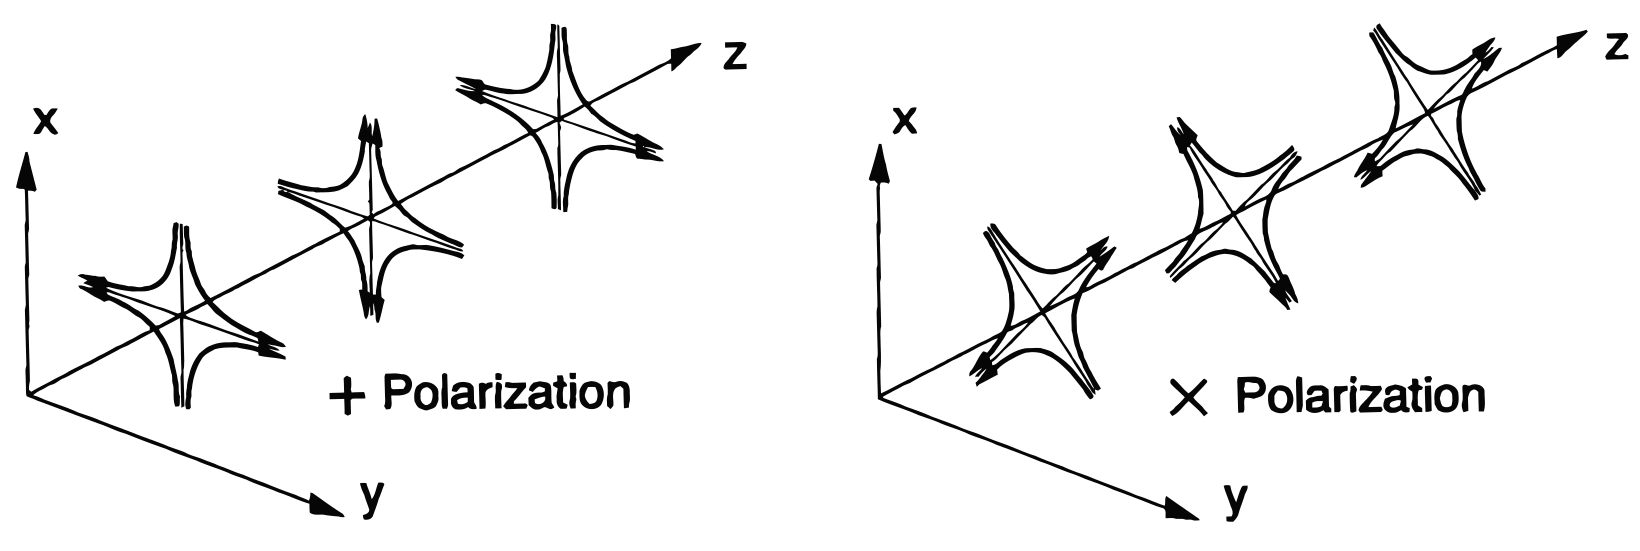
\includegraphics[width=.75\columnwidth]{figs/polarizaciones.png}
\caption{Esquema de lineas de fuerza para las polarizaciones + y $\times$ de una onda que se propaga en la dirección $z$ \cite{Centrella_2010}.}
\label{fig:+x}
\end{figure}


El término $\lambda$ se refiere al conjunto de parámetros que define a la onda producida por la colisión binaria (por ejemplo las masas o spines de los agujeros negros).


\subsection*{Datos Utilizados}

Para esta tesis se utilizaron ondas gravitacionales generadas a partir del modelo híbrido \textit{NRHybSur3dq8}\cite{Varma_2019} que utiliza relatividad numérica y aproximaciones post Newtonianas para colisiones de agujeros negros binarios.
\\

Cada onda generada \( h := h(t; \lambda) := h_{\lambda}(t) := h_{\lambda} \), parametrizada por $\lambda$, se representa con una serie temporal compleja de la forma (ver figura \ref{fig:h_q3})
\[
h = h_+ + ih_{\times}
\]

En el desarrollo de este trabajo \(\lambda\) tendrá 3 dimensiones relevantes, acotadas de la siguiente manera:

\begin{itemize}
\item Relación entre masas $q$: $1 \le q \le 8$
\item Espín del agujero negro más pesado $\chi_{1_Z}$: $|\chi_{1_Z}| < 0.8$
\item Espín del agujero negro más liviano $\chi_{2_Z}$: $|\chi_{2_Z}| < 0.8$
\end{itemize}

Y para tener un espacio de parámetros más simple, en todos los casos se trabajó con $\chi_{1_Z} = \chi_{2_Z}$, por lo que se puede hablar directamente del espín $\chi_{Z}=\chi_{1_Z} = \chi_{1_Z}$. Además se trabajó con el modo $(l, m) =(2, 2)$, pero los resultados obtenidos se pueden aplicar a todos los modos por igual (recordar ecuación \eqref{eq:modes}).

\begin{figure}[h]
\centering
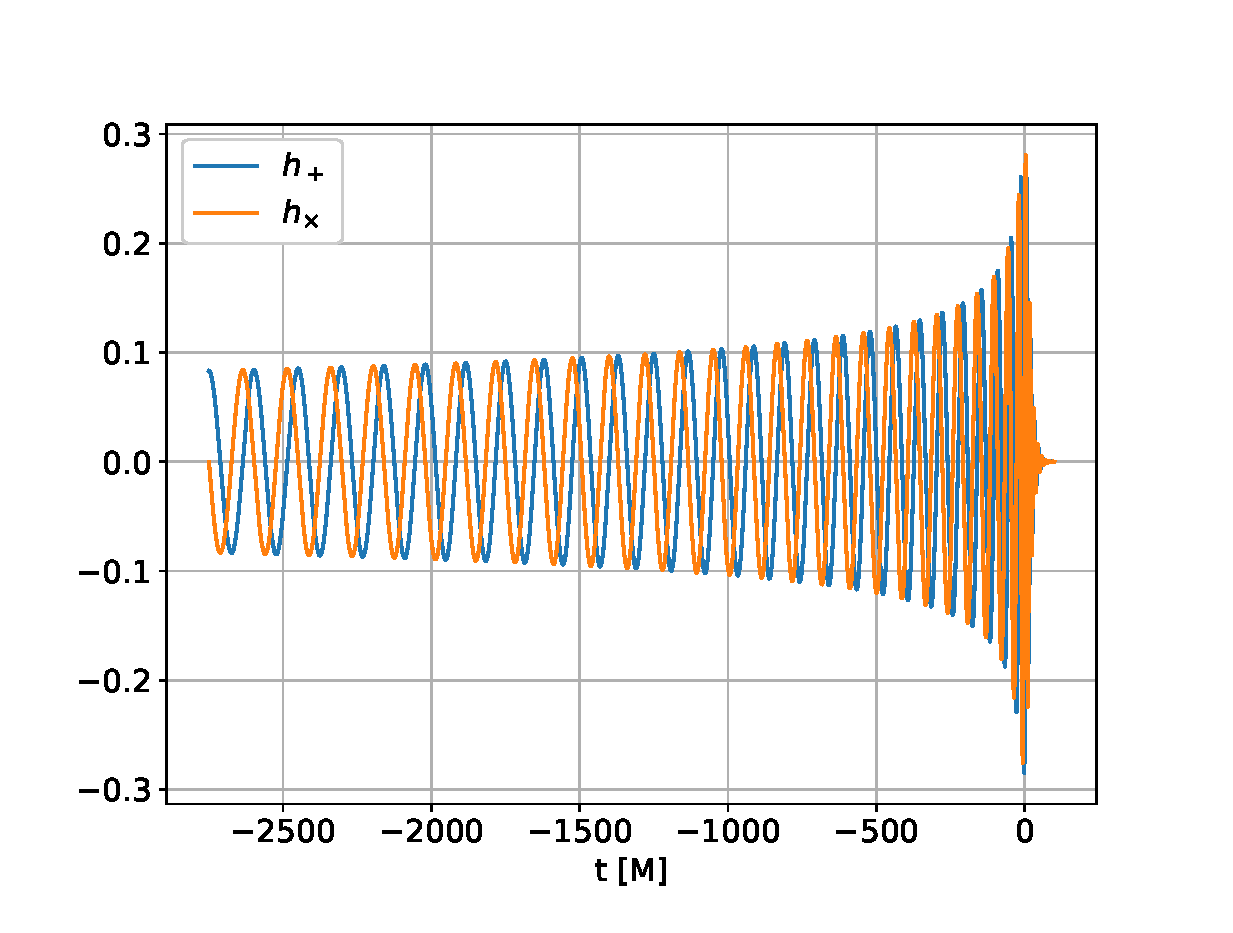
\includegraphics[width=.9\columnwidth]{figs/h_l2m2_q3.eps}
\caption{polarizaciones \(h_+\) y \(h_{\times}\) para $q = 3$, $\chi_{1_Z} = \chi_{2_Z} = 0$, en el modo $l=2$, $m=2$.}
\label{fig:h_q3}
\end{figure}



Se representa un conjunto \( \mathcal{K} \) de N muestras de $\lambda$ de la siguiente forma:

\[ \mathcal{K}  = \{h_{\lambda_i}\}, \hspace{5mm} i = 1, ..., N\]

y debido a que cada $h_{\lambda_i}$ es una serie temporal, se puede representar $\mathcal{K}$ en forma de la matriz $H \in \mathbb{C}^{N\times L}$:

\[
H = 
\begin{bmatrix}
h_{\lambda_1} \\
h_{\lambda_2} \\
 \vdots \\
 h_{\lambda_N} \\
\end{bmatrix}
= 
\begin{bmatrix}
h_{\lambda_1}(t_1) & h_{\lambda_1}(t_2)  & \cdots & h_{\lambda_1}(t_L)\\
 h_{\lambda_2}(t_1) & h_{\lambda_2}(t_2)  & \cdots & h_{\lambda_2}(t_L)\\
 \vdots & \vdots & \ddots &  \vdots \\
h_{\lambda_N}(t_1) & h_{\lambda_N}(t_2)  & \cdots & h_{\lambda_N}(t_L)
\end{bmatrix}
\]

Siendo $L$ la longitud de la serie temporal. De forma que cada fila de $H$ es una onda gravitacional.

También es útil el conjunto de las muestras en el espacio de los parámetros
$\{ \lambda_i \}_{i=1}^N$. 
Un conjunto de entrenamiento (o validación) consistirá en el conjunto que contenga cada parámetro $\lambda_i$ junto con su onda parametrizada $h_{\lambda_i}$:

\[
\mathcal{T} := \{ \lambda_i, h_{\lambda_i} \}_{i=1}^N
\]



